\documentclass[Thesis.tex]{subfiles}
\begin{document}
\setkeys{Gin}{draft=false}
\chapter{{\sc VaryLab} - Discrete surface optimization}
\label{chp:varylab}

\section{Introduction}

{\sc VaryLab} is a software developed at Berlin Institute of Technology by the author, Thilo R\"orig, and others. It is supported by DFG SFB/TRR 109 Discretization in Geometry and Dynamics. It is designed to be an extensible and modular tool for experiments with discrete surfaces in pure mathematics and applications in industrial geometry. {\sc VaryLab} is used to create the result in Chapters~\ref{chp:periodic_conformal_maps}, \marginpar{bullshit!}\ref{chp:quasiisothermic}, and \ref{chp:gridshells}.

In its core {\sc VaryLab} is a solver for non-linear optimization problems on the coordinates of a given 3D discrete surface. That means given a surface $S$ and functionals $f_1,\ldots,f_n:S\to\R$ we (try to) minimize the combined functional

\begin{eqnarray*}
	f(S) = \sum_{i=1}^n \lambda_i f_i(S)
\end{eqnarray*}
where $\lambda_1,\ldots,\lambda_n\in \R$ are user defined weights. Correspondingly the first and second  derivatives of $f_i(S)$ are weighted by $\lambda_i$
\begin{eqnarray*}
	\nabla f(S) = \sum_{i=1}^n \lambda_i \nabla f_i(S), \quad \nabla\nabla f(S) = \sum_{i=1}^n \lambda_i \nabla\nabla f_i(S).
\end{eqnarray*}

{\sc VaryLab} uses the numerical library {\sc PETSc}/{\sc TAO} \cite{petsc-user-ref, petsc-web-page, tao-user-ref} and the corresponding {\sc Java} bindings \cite{jpetsctao-web-page} for computations. To run optimization methods we need at least an implementation of the functional's value. Other methods need gradient or Hessian of the functional. The most important methods are
 
\begin{tabular}{c | c | c}
	$f$ & $f$, $\nabla f$ & $f$, $\nabla f$, $\nabla\nabla f$\\ \hline
	{\tt NM} Nelder-Mead & {\tt LMVM} Limited-Memory, Variable-Metric & {\tt NLS} Newton Line-Search \\
	& {\tt CG} Conjugate Gradient & {\tt NTR} Newton Trust-Region.
\end{tabular}

In {\sc VaryLab} a functional can choose to implement just the value, see Section~\ref{sec:plugin-api}. Additionally it can implement the gradient and the Hessian of $S$. In principle all methods can be used with all functionals even if those do not implement all data needed for the algorithm. {\sc VaryLab} approximates the values of the gradient or the Hessian if they are missing. 

Derivatives and numerical substitutes, 
Boundary Conditions
Numerics
Build-In Functionals
Plug-in facility and extensibility, 
Data Visualization (scalar, vector)
Remeshing

\begin{figure}
\begin{center}
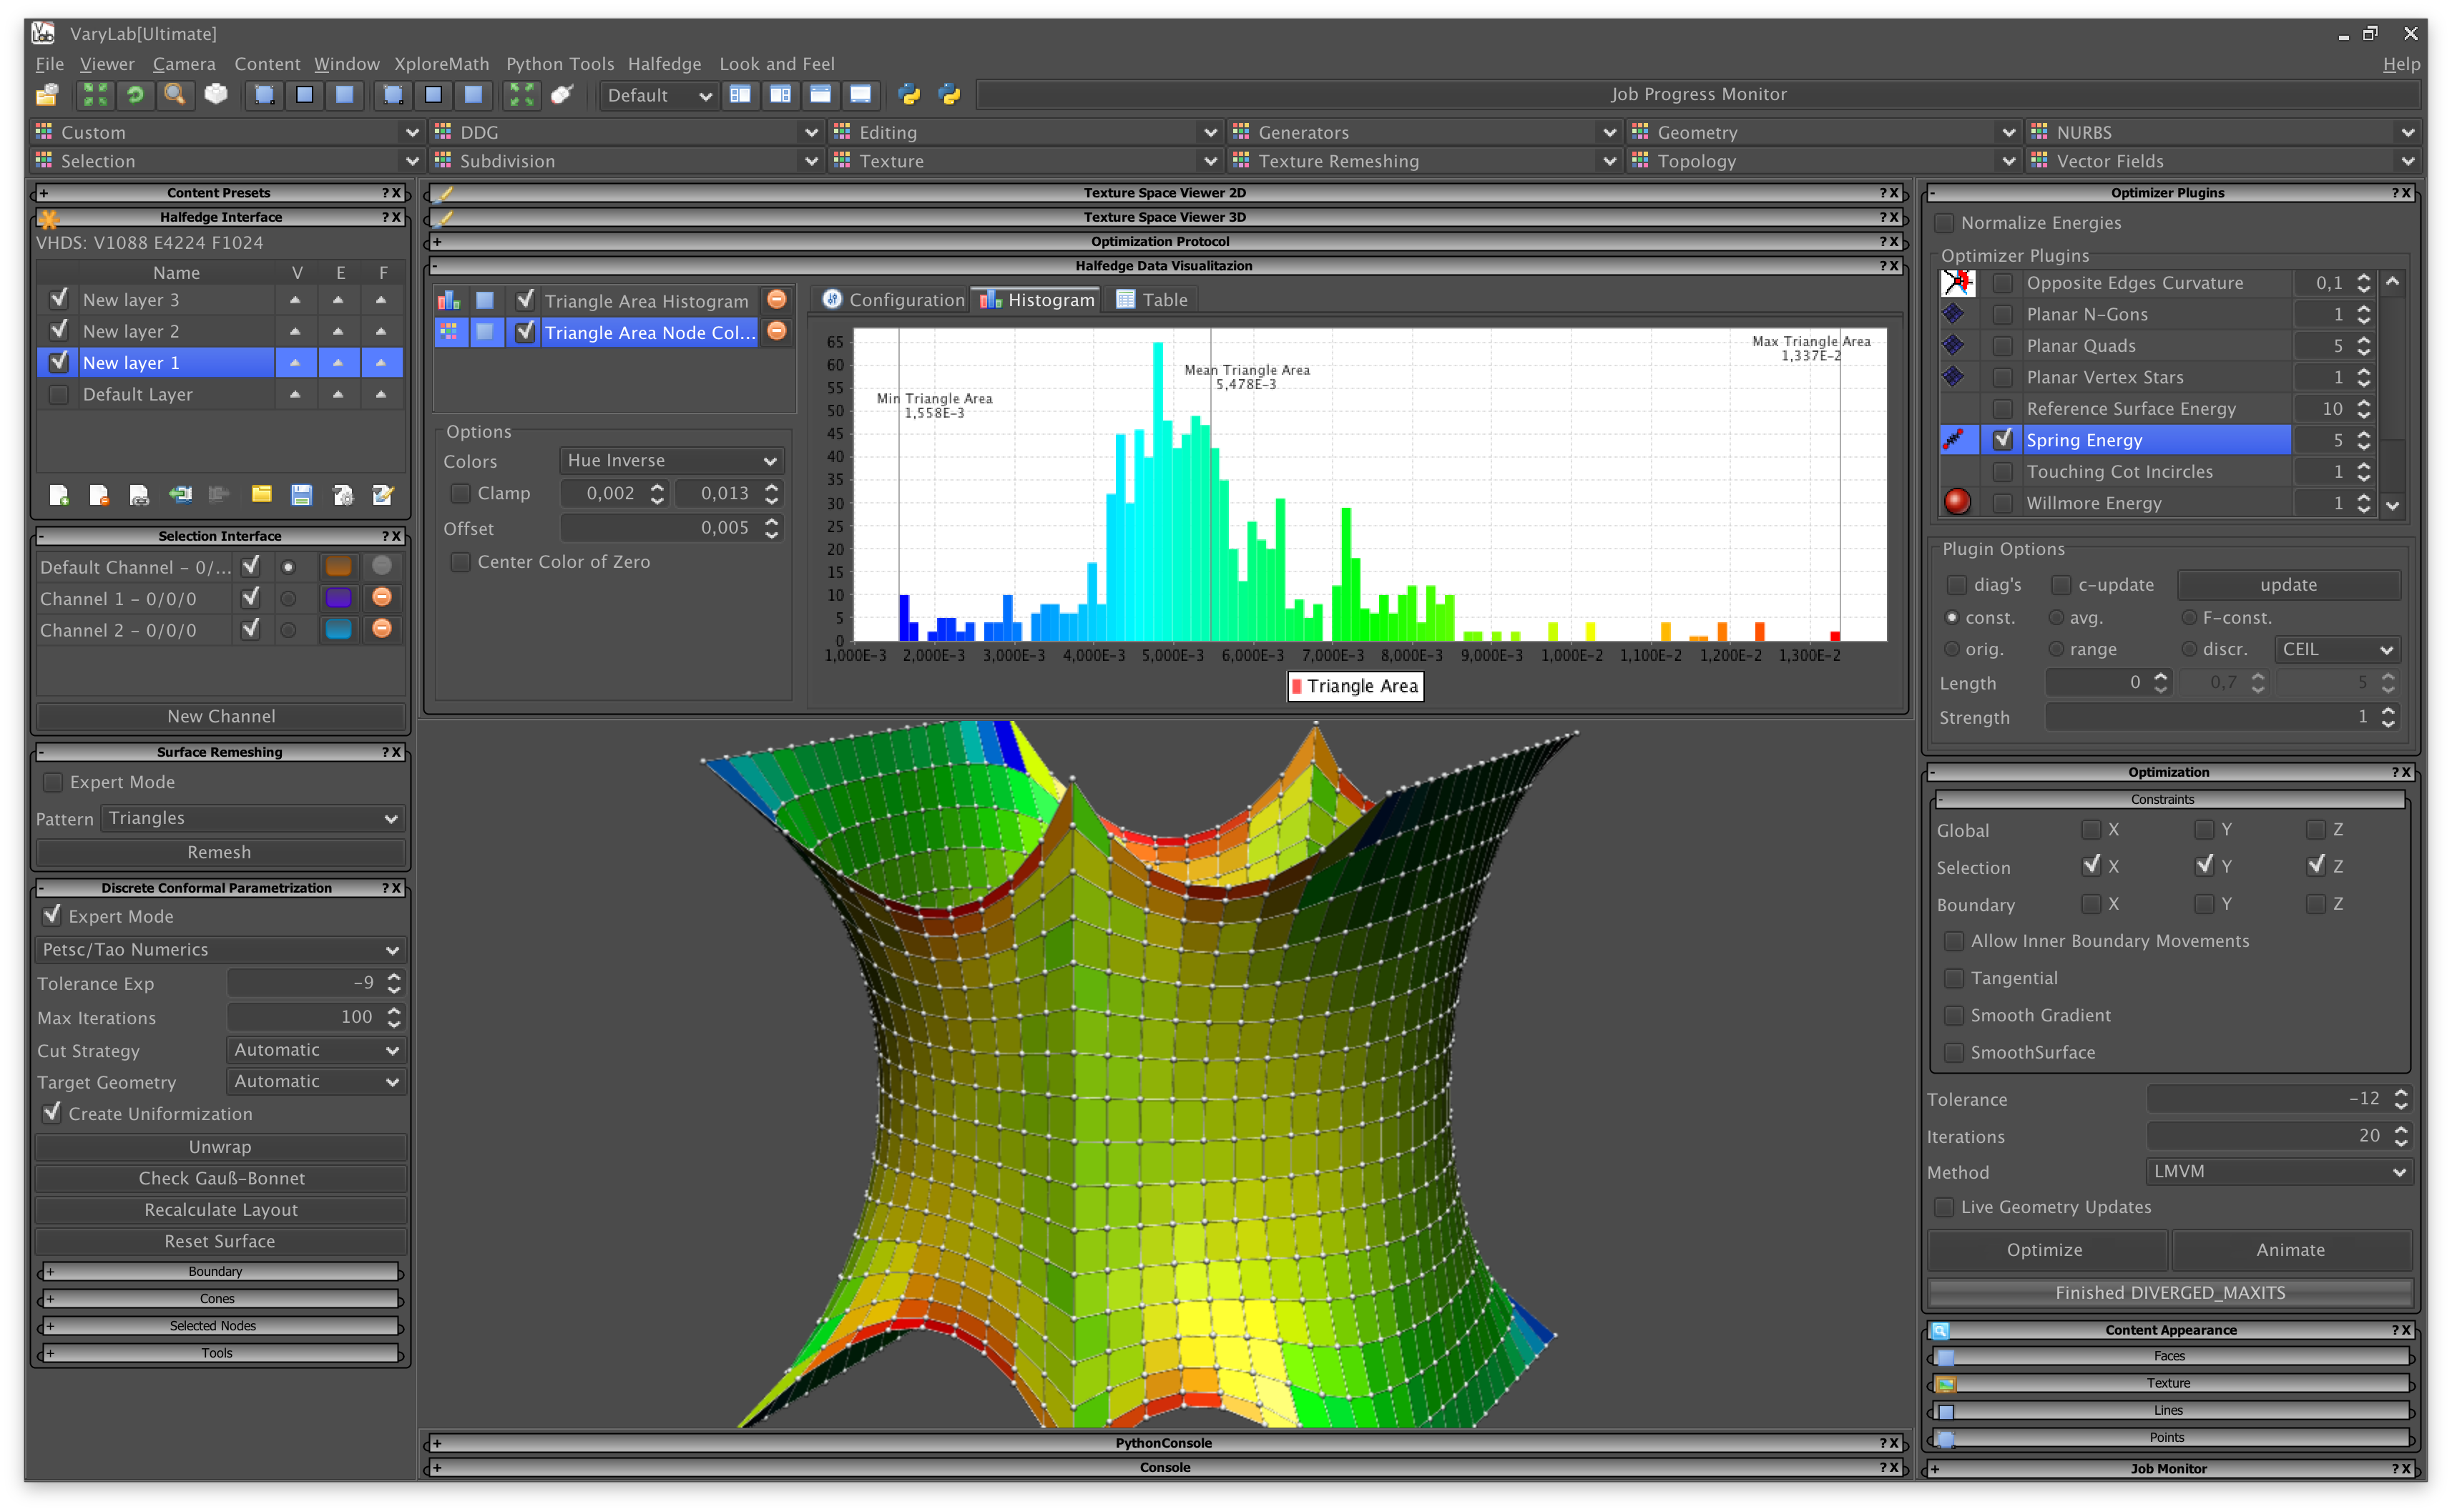
\includegraphics[width=\textwidth]{varylab/varylab_main.png}
\caption{{\sc VaryLab} user interface.}
\label{fig:varylab_main_ui}
\end{center}
\end{figure}

\section{Plug-in API}
\label{sec:plugin-api}

\section{User interface}

\begin{figure}
\begin{center}
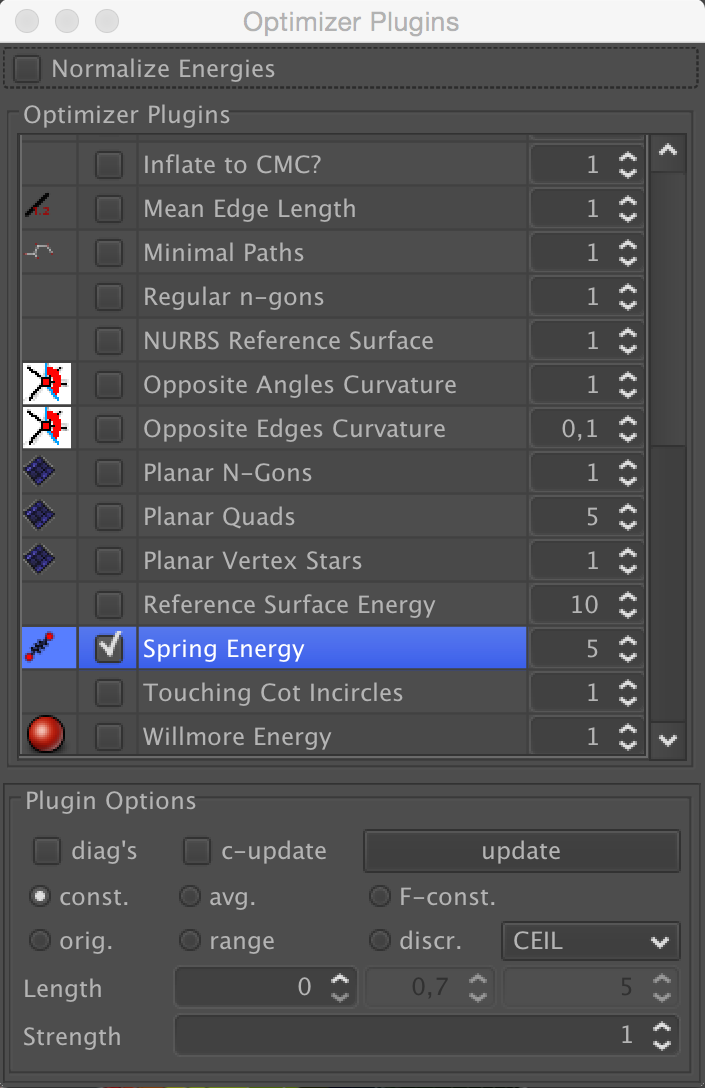
\includegraphics[width=0.5\textwidth]{varylab/optimization_plugins.png}\hfill
\begin{minipage}[b]{0.47\linewidth}
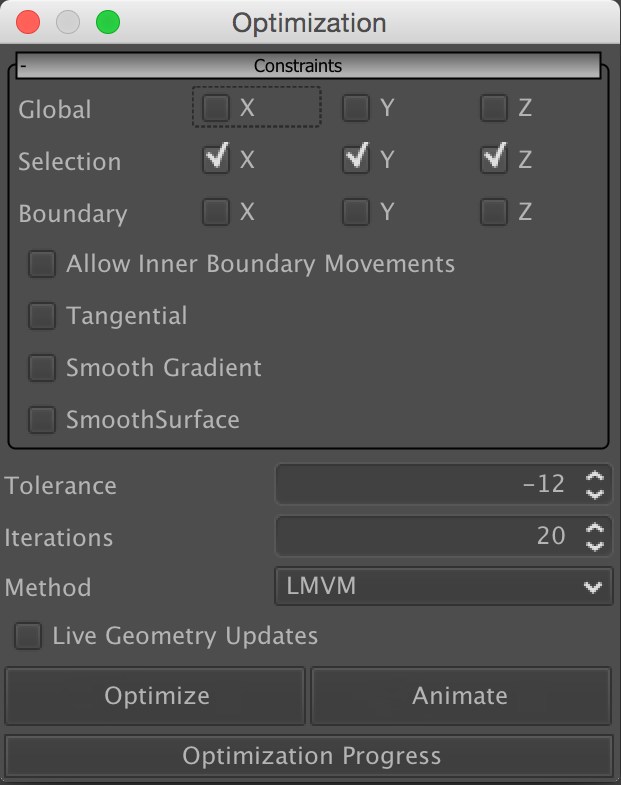
\includegraphics[width=\linewidth]{varylab/optimization.png}\\
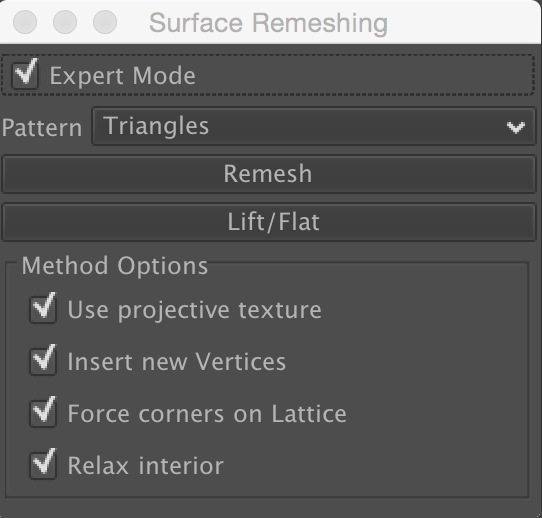
\includegraphics[width=\linewidth]{varylab/remeshing.png}
\end{minipage}\\
\vskip 0.05cm
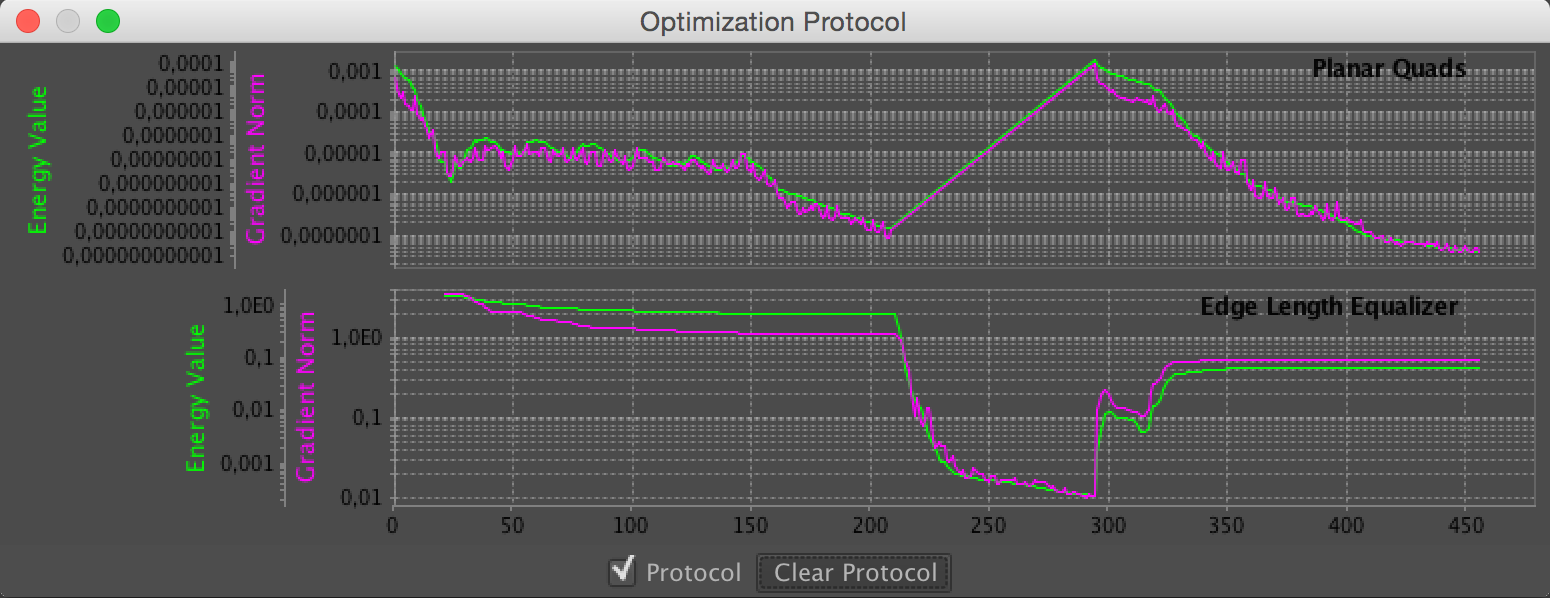
\includegraphics[width=\textwidth]{varylab/protocol.png}
\caption{The main user interface panels of {\sc VaryLab}. List of optimization functional plug-ins and their options (left). Main optimization controls with global constraints and minimizer settings (top right). Remeshing ui for different patterns (right middle). Optimization protocol panel (bottom) shows the progress of the optimization for each activated energy.}
\label{default}
\end{center}
\end{figure}


\section{Periodic conformal maps with {\sc VaryLab}}
In this section we describe how the methods of Chapter~\ref{chp:periodic_conformal_maps} are implemented in {\sc VaryLab}. We split the process in two parts. Part one describes the creation of periodic triangle, quad, or hexagonal meshes from an initial unstructured triangle mesh. Part two deals with optimization of panels created from a mesh in part one.

\subsection{Periodic meshes}
The parameterization part of the work is carried out via the {\sc ConformalLab} main user interface. 

\begin{figure}
\resizebox{\textwidth}{!}{
	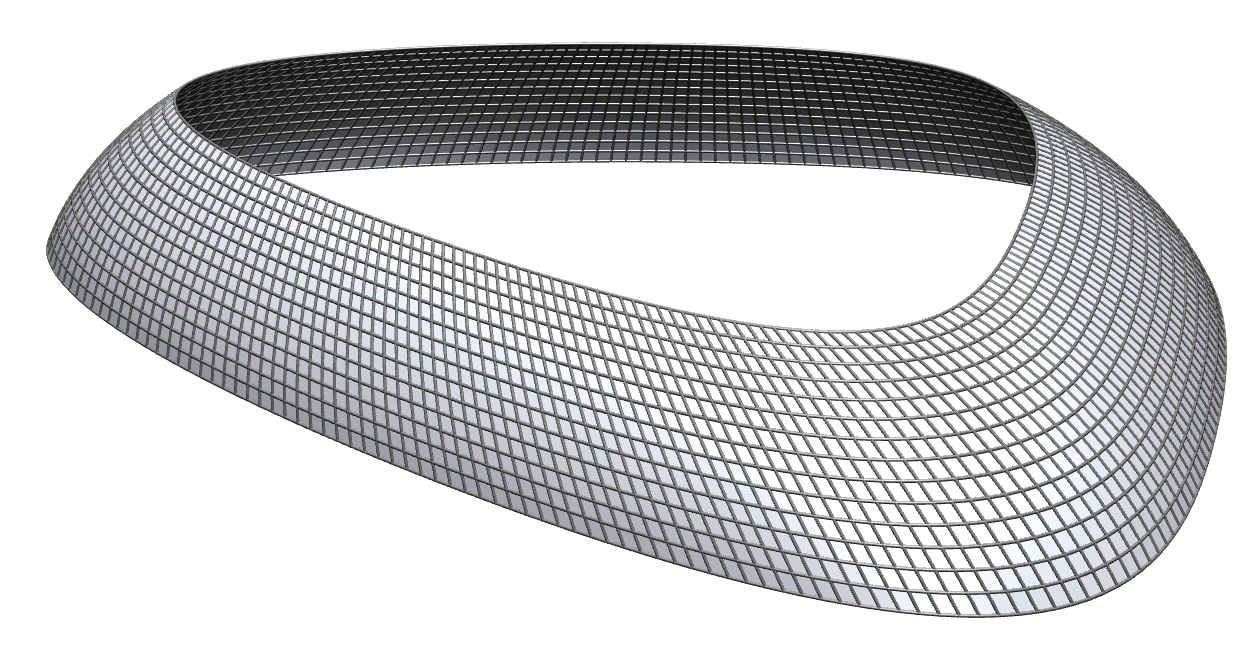
\includegraphics{periodic/step00.png}
	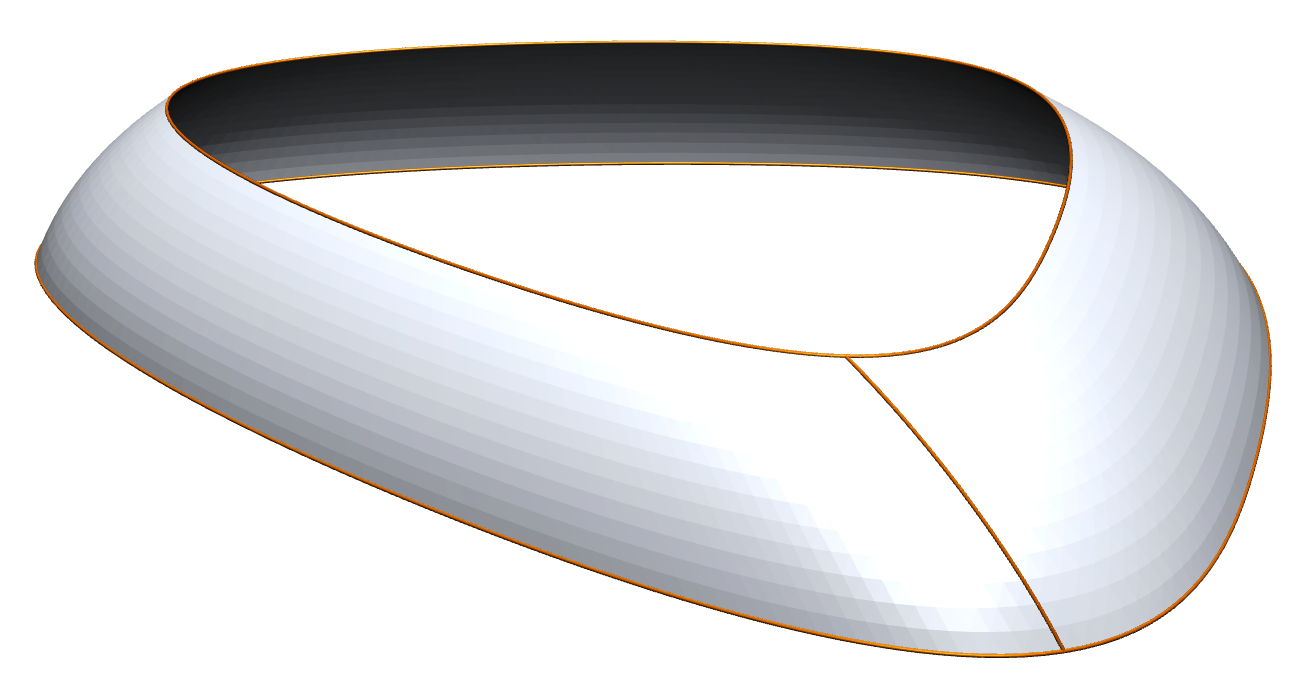
\includegraphics{periodic/step01_surface.png}	
	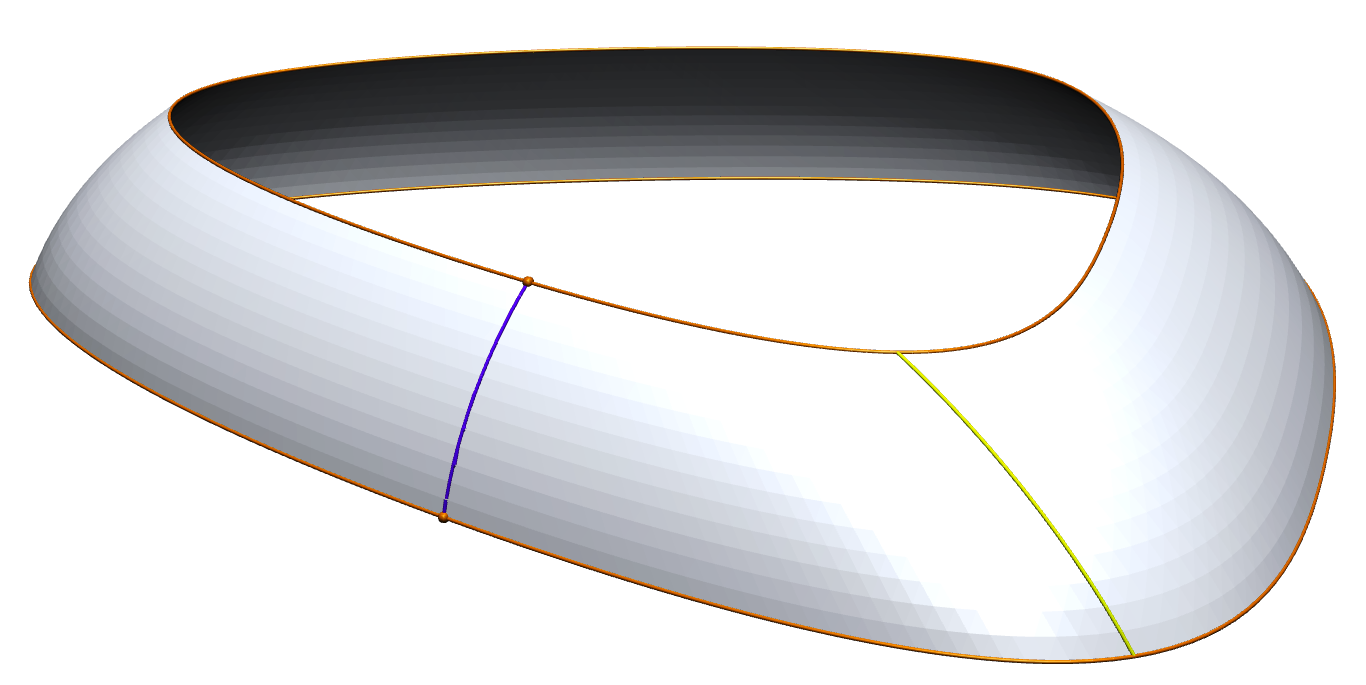
\includegraphics{periodic/step02_surface.png}		
}
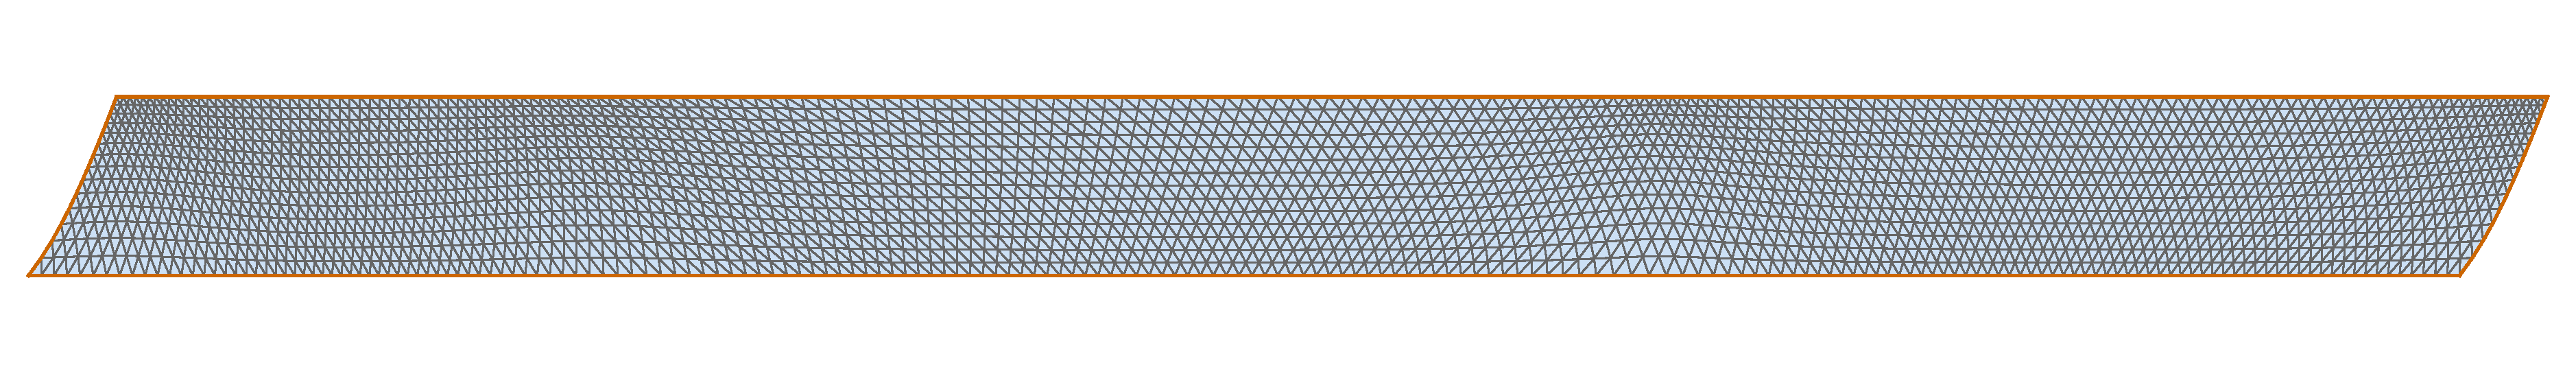
\includegraphics[width=\textwidth]{periodic/step01_map.pdf}
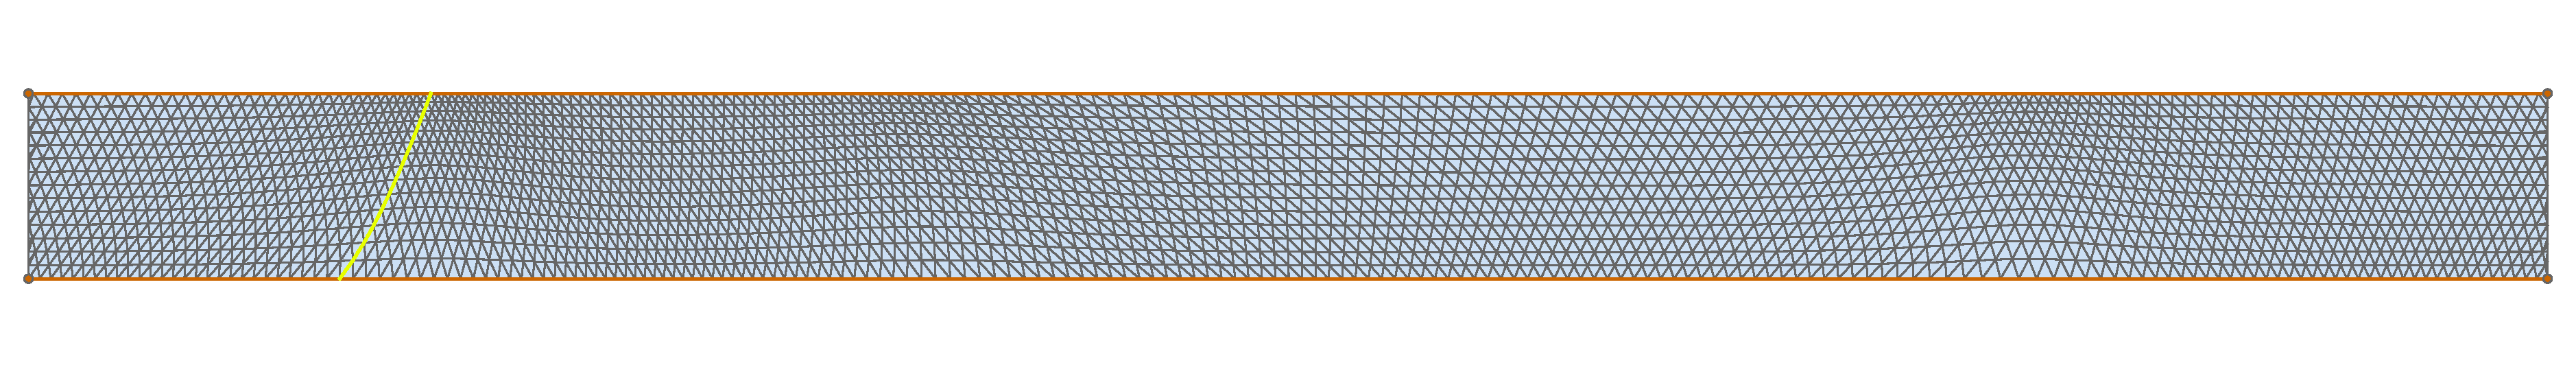
\includegraphics[width=\textwidth]{periodic/step02_map.pdf}	
\resizebox{\textwidth}{!}{
	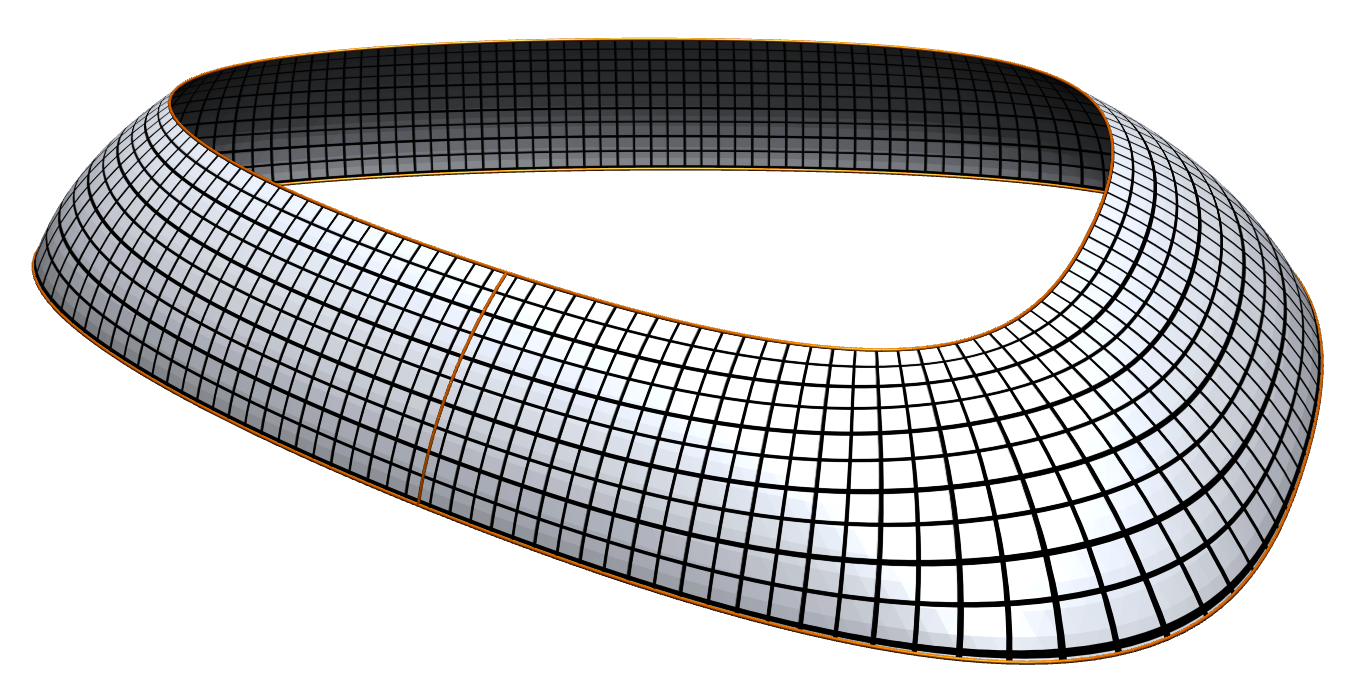
\includegraphics{periodic/step03_quads.png}
	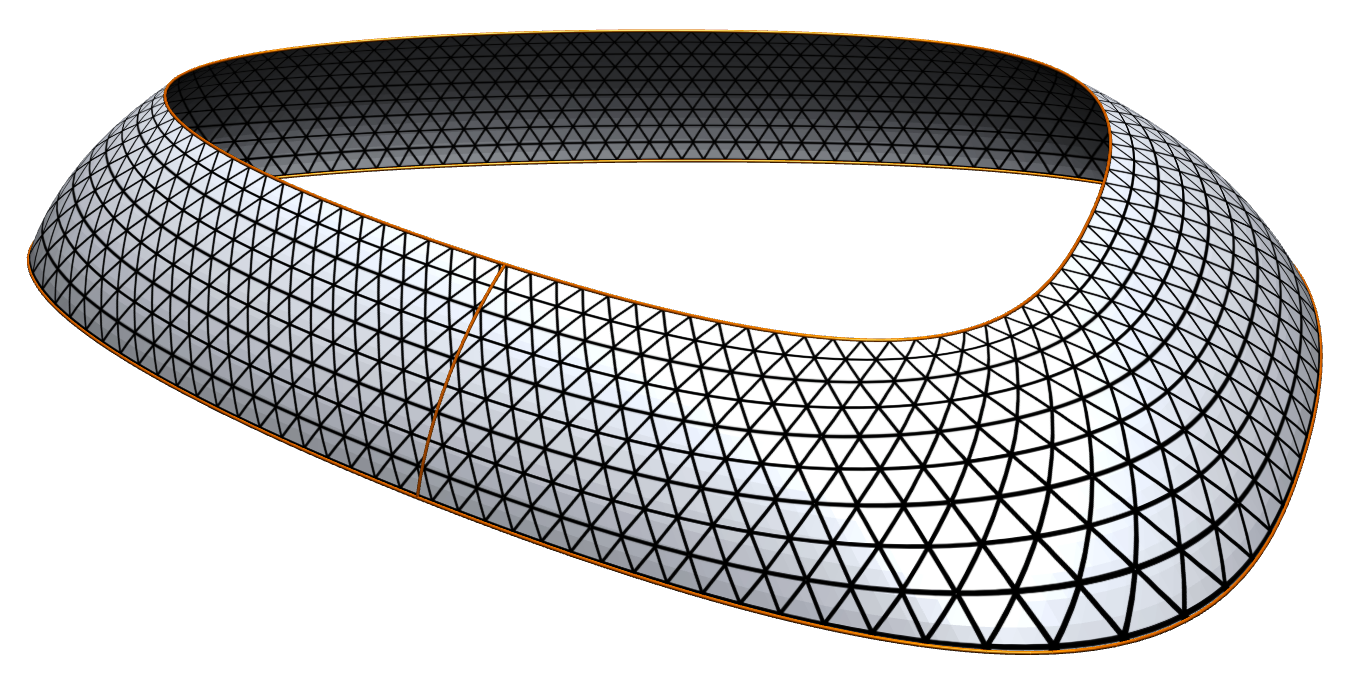
\includegraphics{periodic/step03_triangles.png}
}
\resizebox{\textwidth}{!}{
	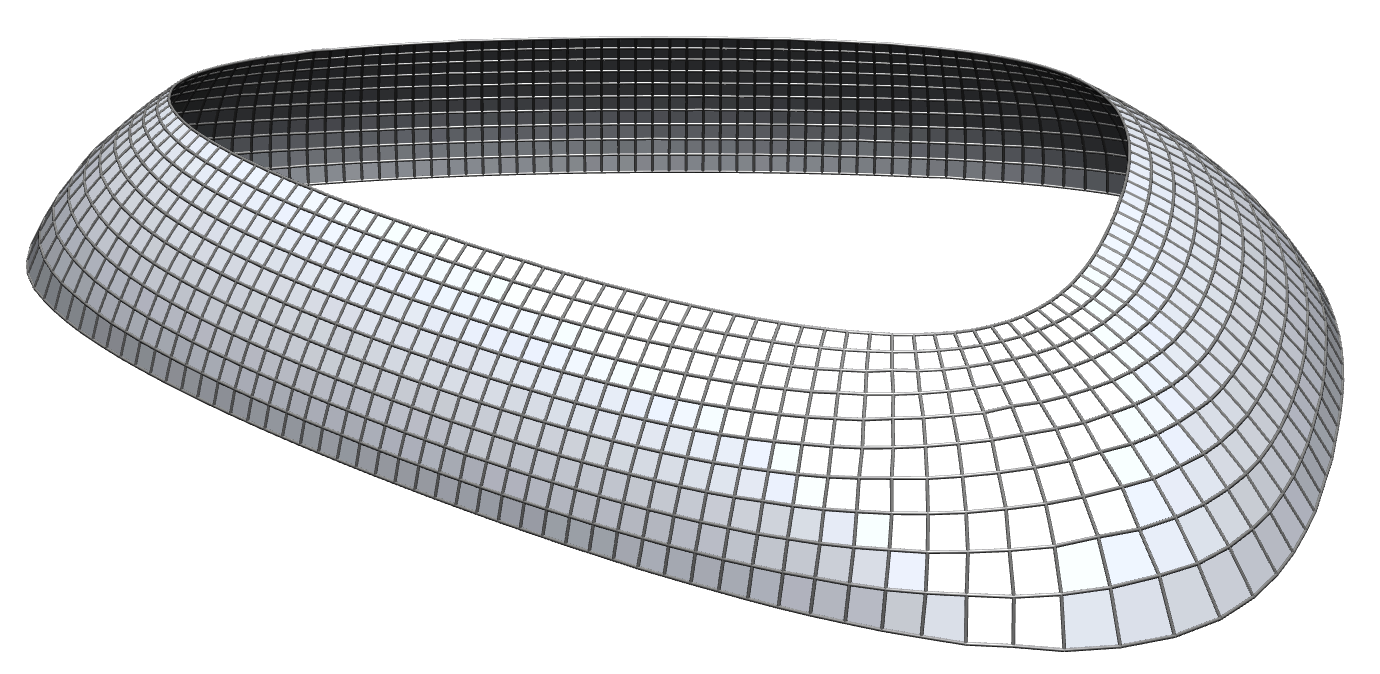
\includegraphics{periodic/step04_quads_surface.png}
	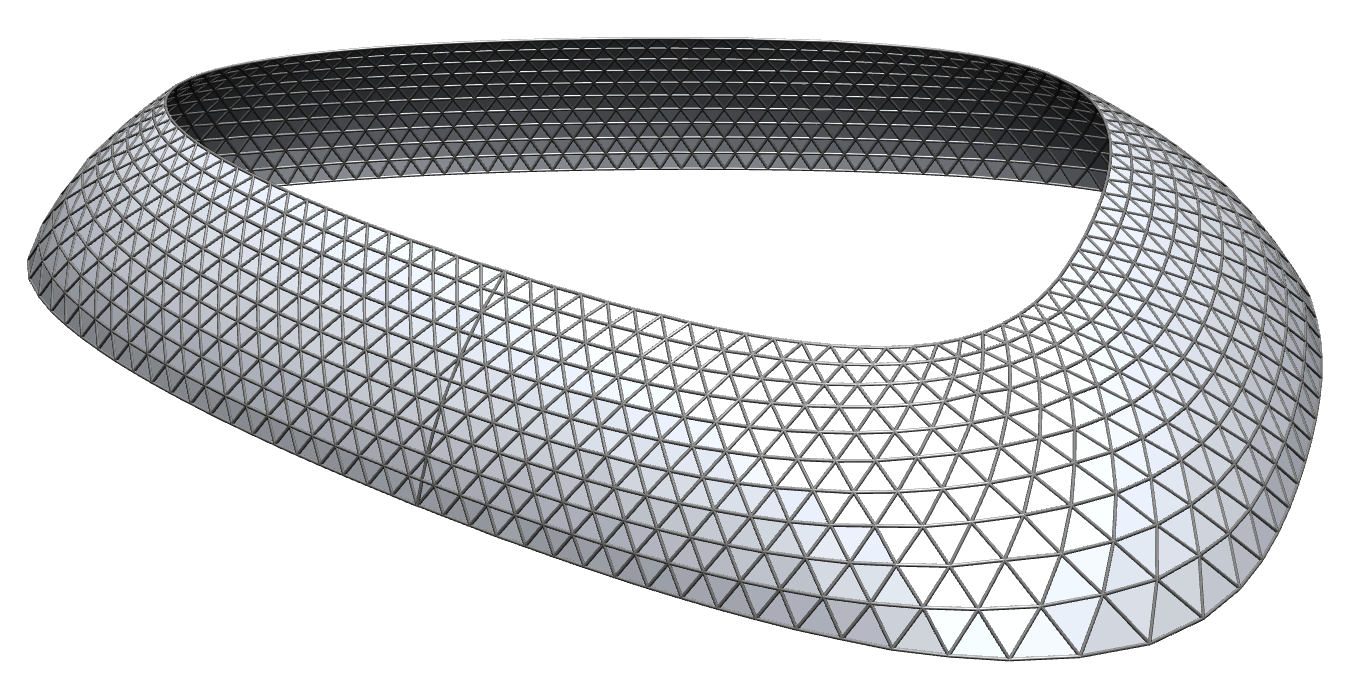
\includegraphics{periodic/step04_triangles_surface.png}
}
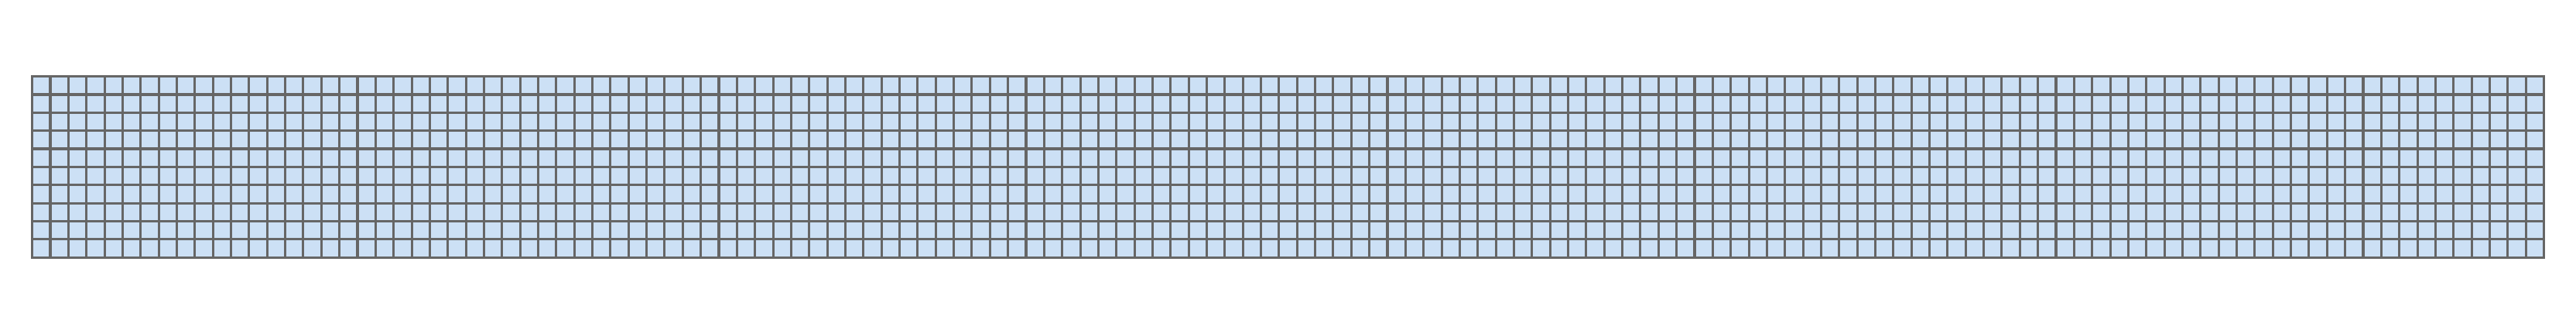
\includegraphics[width=\textwidth]{periodic/step04_quads_map.pdf}
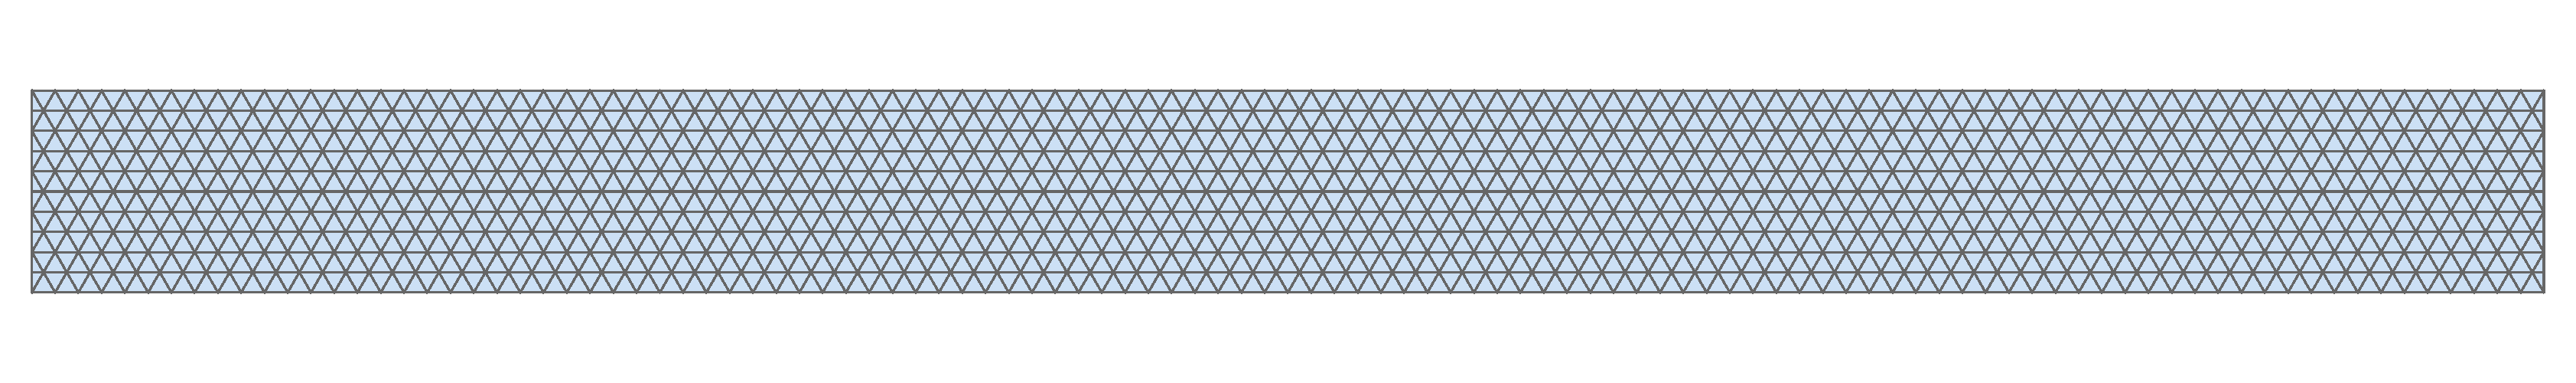
\includegraphics[width=\textwidth]{periodic/step04_triangles_map.pdf}	
\resizebox{\textwidth}{!}{
	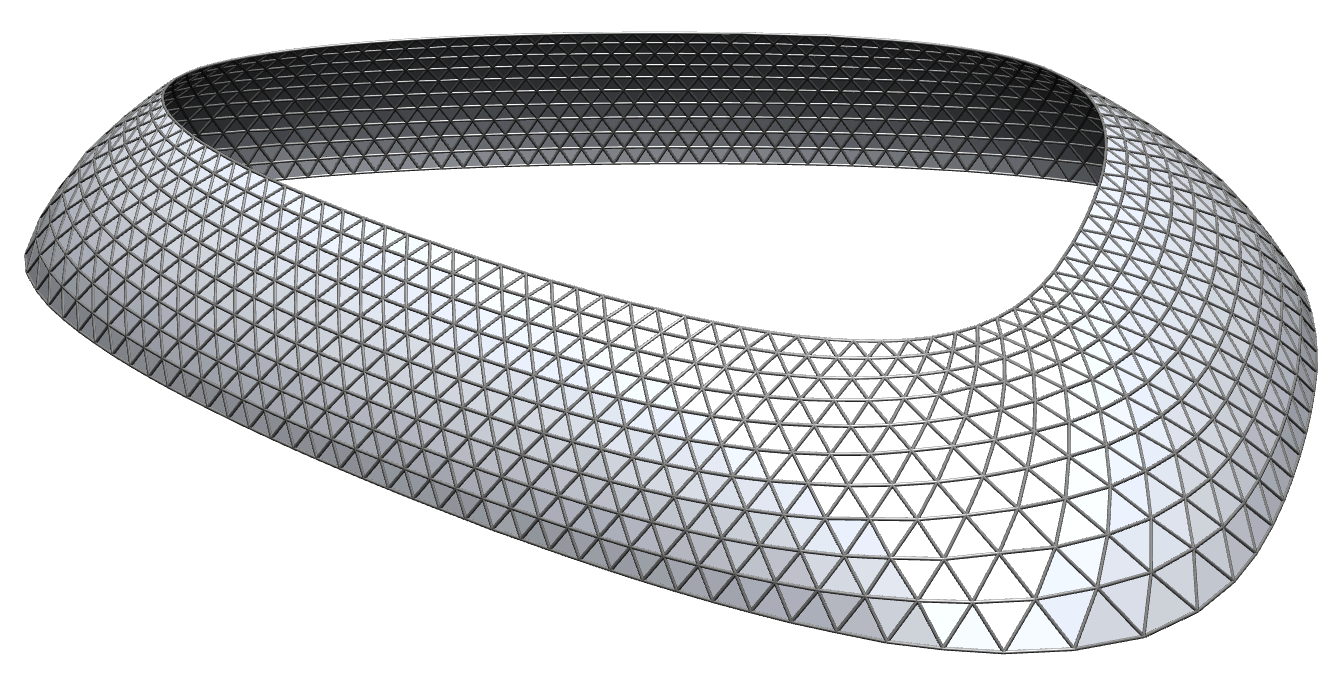
\includegraphics{periodic/step05.png}
	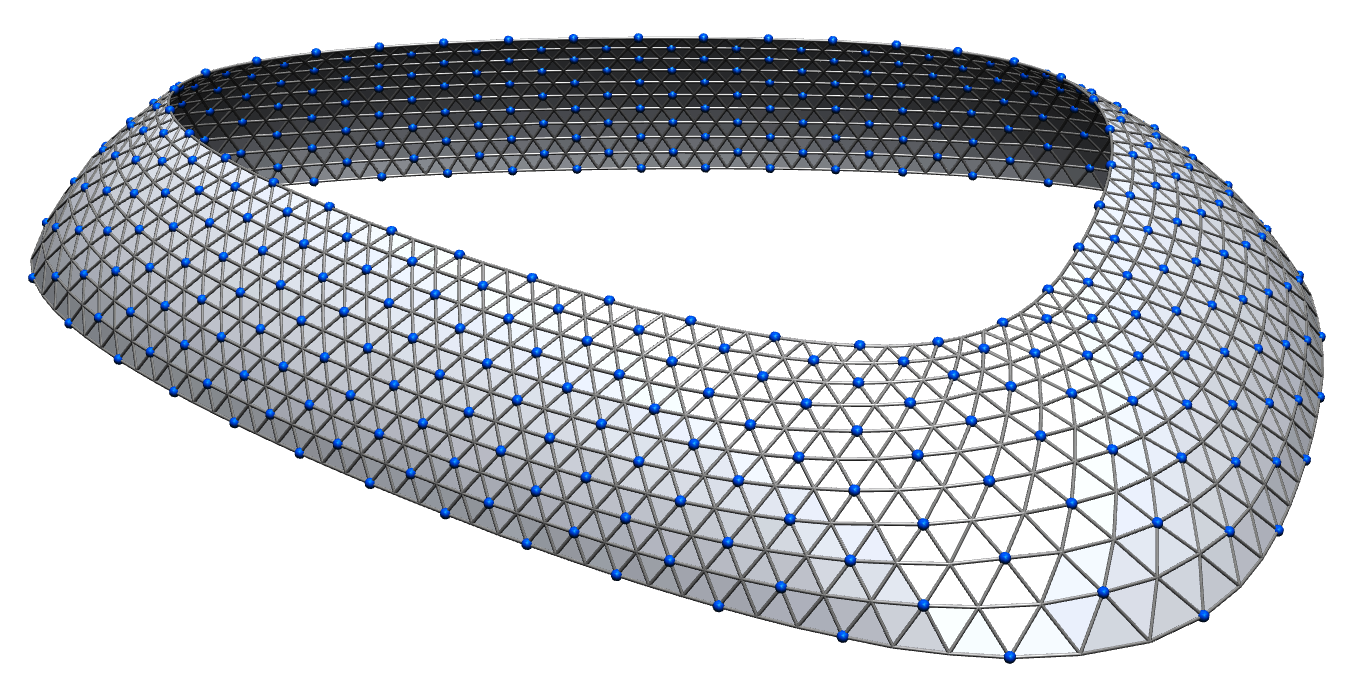
\includegraphics{periodic/step06.png}
	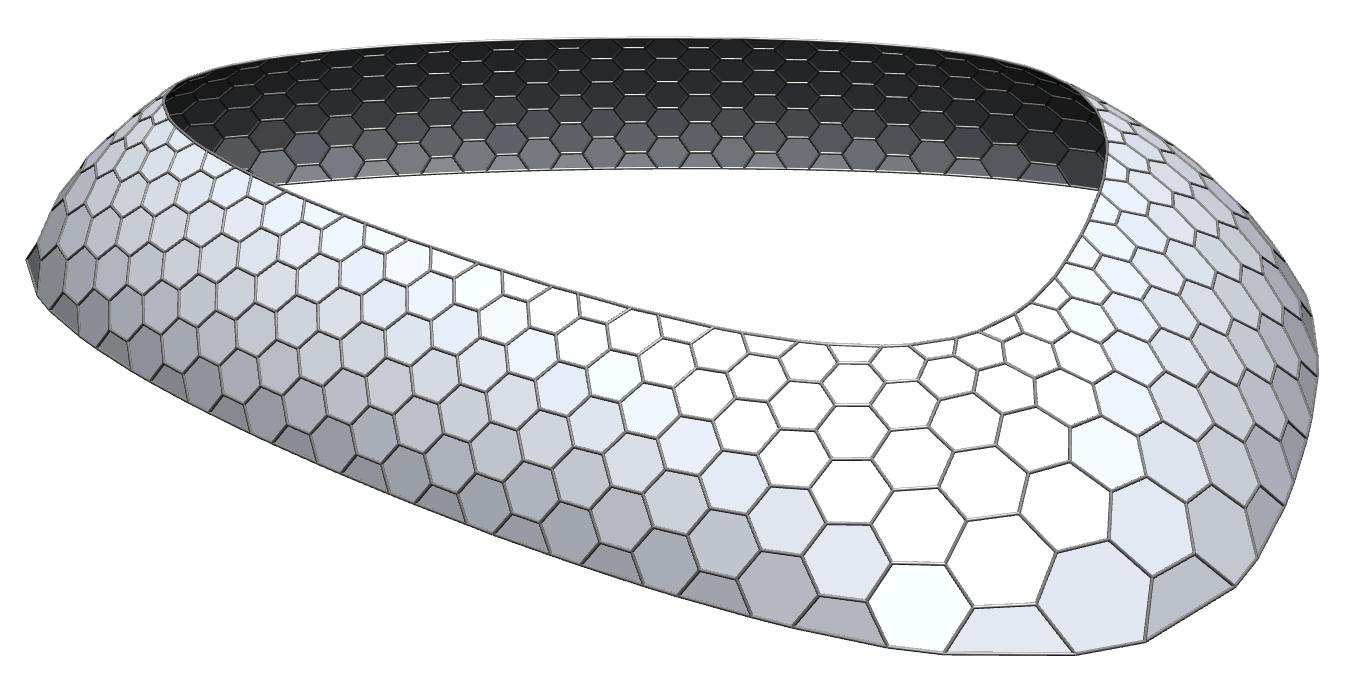
\includegraphics{periodic/step07.png}	
}
\caption{Periodic patterns via periodic conformal maps.}
\label{fig:periodic_algorithm}
\end{figure}

\subsection{Panel optimization}

\begin{itemize}
\item[0] Load a surface with two boundary component.
\item[1] Create a conformal parameterization with straight boundary. A cut is introduced to uniquely define the map.
\item[2] Use the [Cut and Glue Texture Domain] command and select [Orthogonal to Boundary] to create a map to a rectangle.
\item[3] Select a predefined texture for quad or triangle mesh preview.
\item[4] Perform remeshing either for [Boundary Aligned Triangles] or [Boundary Aligned Quads]
\item[5] Create a watertight mesh using the [Watertight Mesh Generator] and remove extra edges and vertices.
\item[6] For hexagonal mesh creation select from the periodic triangle mesh all centers of hexagons. 
\item[7] Use the [Remove Vertex and Fill] command to create a periodic hexagonal mesh.
\end{itemize}

\begin{figure}
\resizebox{\textwidth}{!}{
	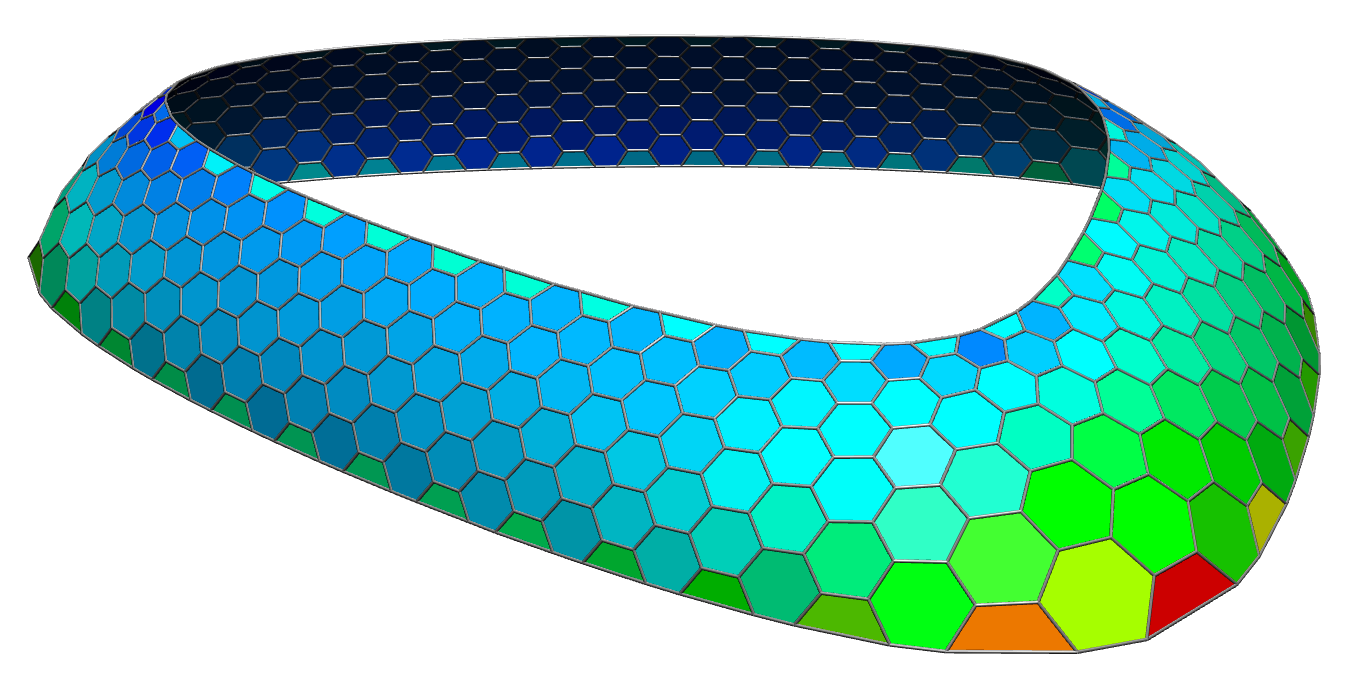
\includegraphics[width=5cm]{periodic/step08_surface.png}
	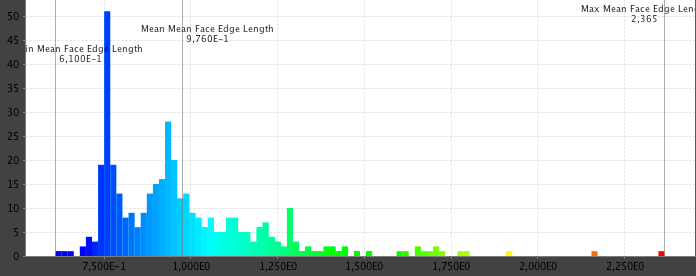
\includegraphics[width=5cm]{periodic/step08_histogram.png}		
}
\resizebox{\textwidth}{!}{
	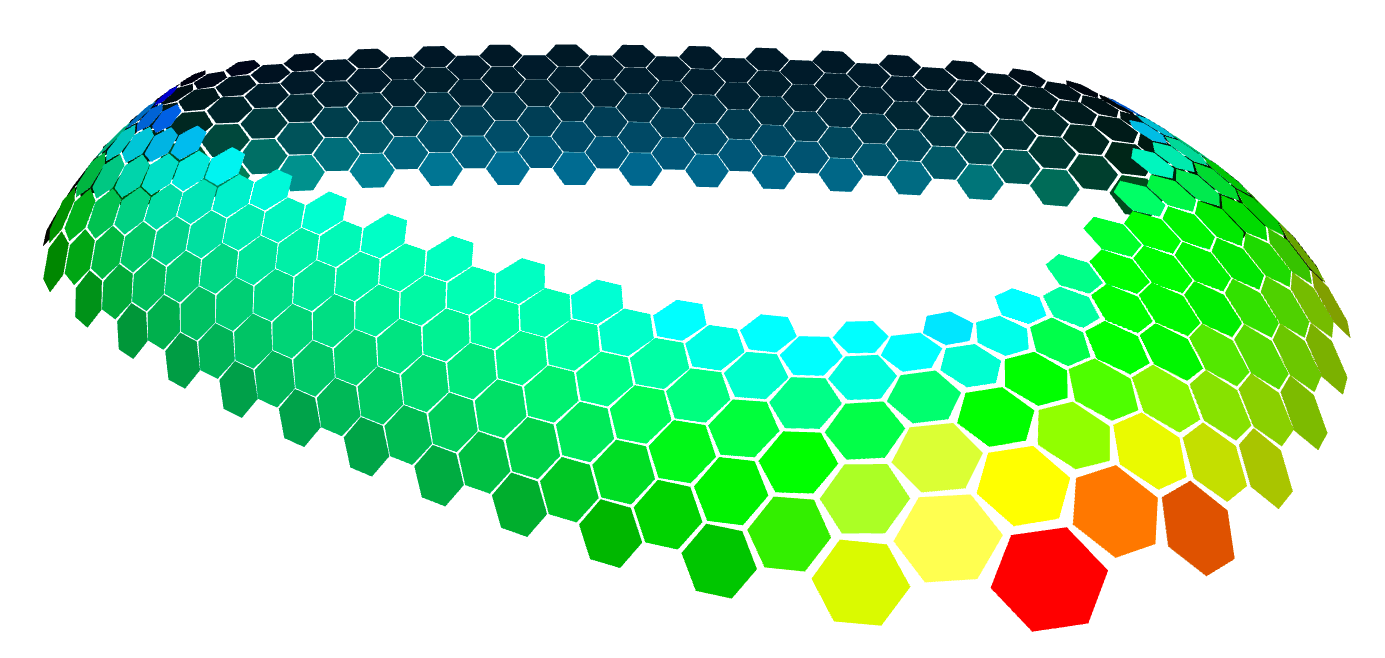
\includegraphics[width=13cm]{periodic/step09_surface.png}
	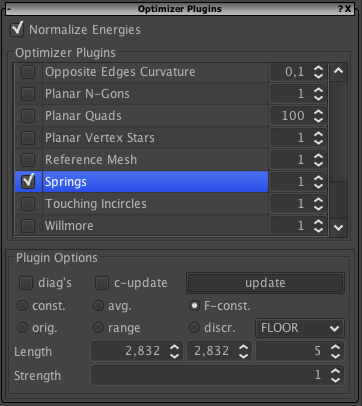
\includegraphics[width=5cm]{periodic/step09_fconst.png}
}
\resizebox{\textwidth}{!}{
	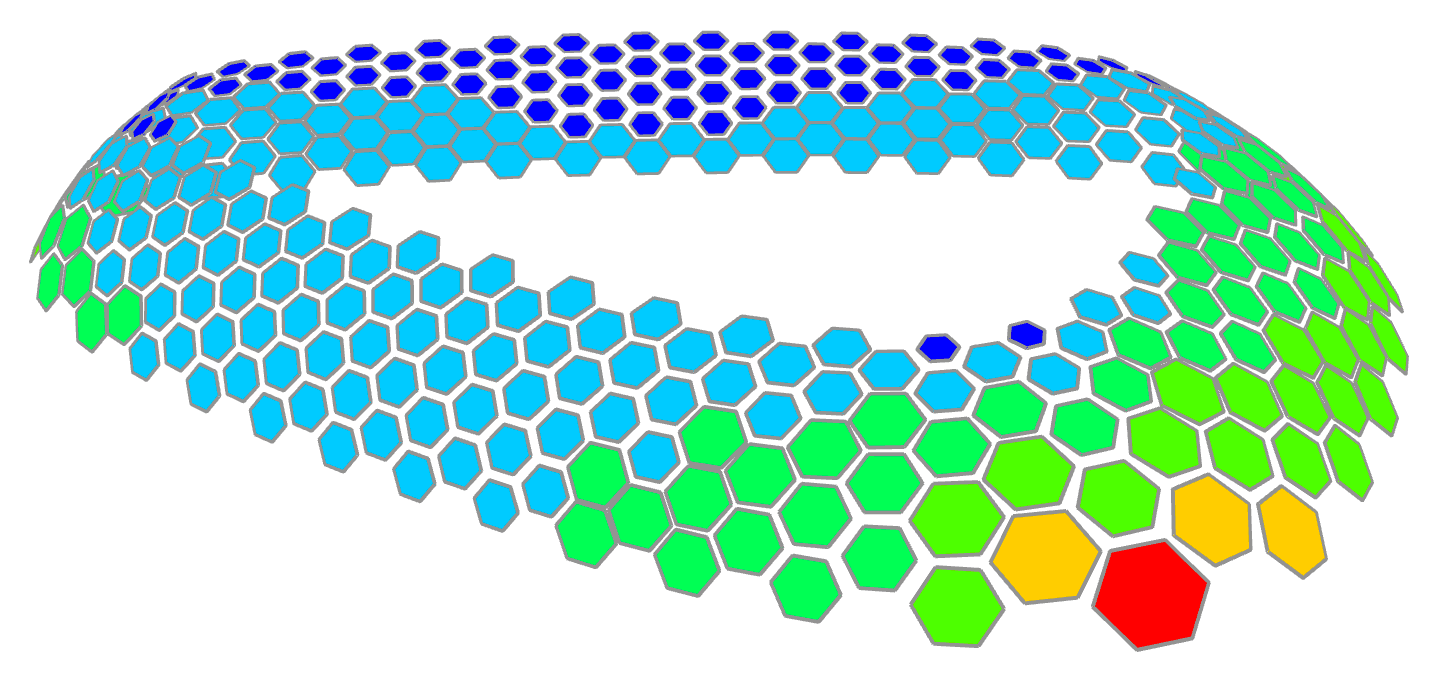
\includegraphics[width=13cm]{periodic/step11_surface1.png}
	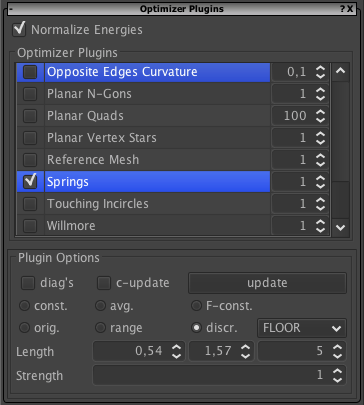
\includegraphics[width=5cm]{periodic/step10_springs.png}
}
\caption{Quantized panelization}
\label{fig:quantization_algorithm}
\end{figure}



\begin{itemize}
\item[8] [Topology]->[Explode] creates separate faces. Use a [Mean face Edge Length] histogram to show the density of edge lengths. If you want planar panels you should planarize them now. 
\item[9] Equalize the edge lengths per face using the [Springs] Energy and [F-const] option. Use the [Floor] rounding method. Press [Update] to set target lengths per face.
\item[10] From the histogram read off the smallest and largest edge lengths and transfer those into the [Springs] energy ui. Select the [discr.] option and the number of discrete steps.
\item[11] Optimize the surface to consist of a limited number of panel sizes.
\end{itemize}


Load a model with two boundary components. 

\section{Quasiisothermic meshes with {\sc VaryLab}}

\section{Gridshell creation using {\sc VaryLab}}

\subfilebibliography
\end{document}

%%% Local Variables:
%%% TeX-master: "Thesis.tex"
%%% End: